\chapter{Uruchomienie i weryfikacja poprawności działania systemu}

Celem niniejszego rozdziału jest opisanie procesu uruchomienia systemu i weryfikacji poprawności działania, poprzez sprawdzenie połączeń między węzłami sieci Thread oraz zasad działania systemu, przedstawionych w podsekcji \ref{subsec:system-behaviour}.

\section{Uruchomienie}

Pierwszym krokiem w uruchomieniu systemu jest utworzenie sieci Thread. Proces tworzenie topologii rozpoczęto od wystartowania aplikacji OTBR.

Podłączono zaprogramowaną platformę, jak omówiono w Podsekcji \ref{subsec:otbr-implementation}, do portu szeregowego urządzenia gospodarza, a następnie sprawdzono poprawność komunikacji między maszyną wirtualną a urządzeniem pracującym jako RCP. Ostatecznie uruchomiono kontener Docker, zawierający aplikację OTBR, wykorzystując przygotowany wcześniej skrypt \textit{my-run-otbr.sh} znajdujący się w repozytorium \cite{project-repo}. Upewniwszy się o poprawnym działaniu Rutera Brzegowego, rozpoczęto tworzenie sieci Thread.
    
Do konfiguracji sieci wykorzystano interfejs graficzny OTBR Web GUI, będący serwisem zapewnionym w ramach aplikacji OTBR. Zrzut ekrany przedstawiającego wymieniony interfejs graficzny, zaprezentowano na Rysunku \ref{fig:otbr-web-gui}.

\begin{figure}[H]
    \centering
    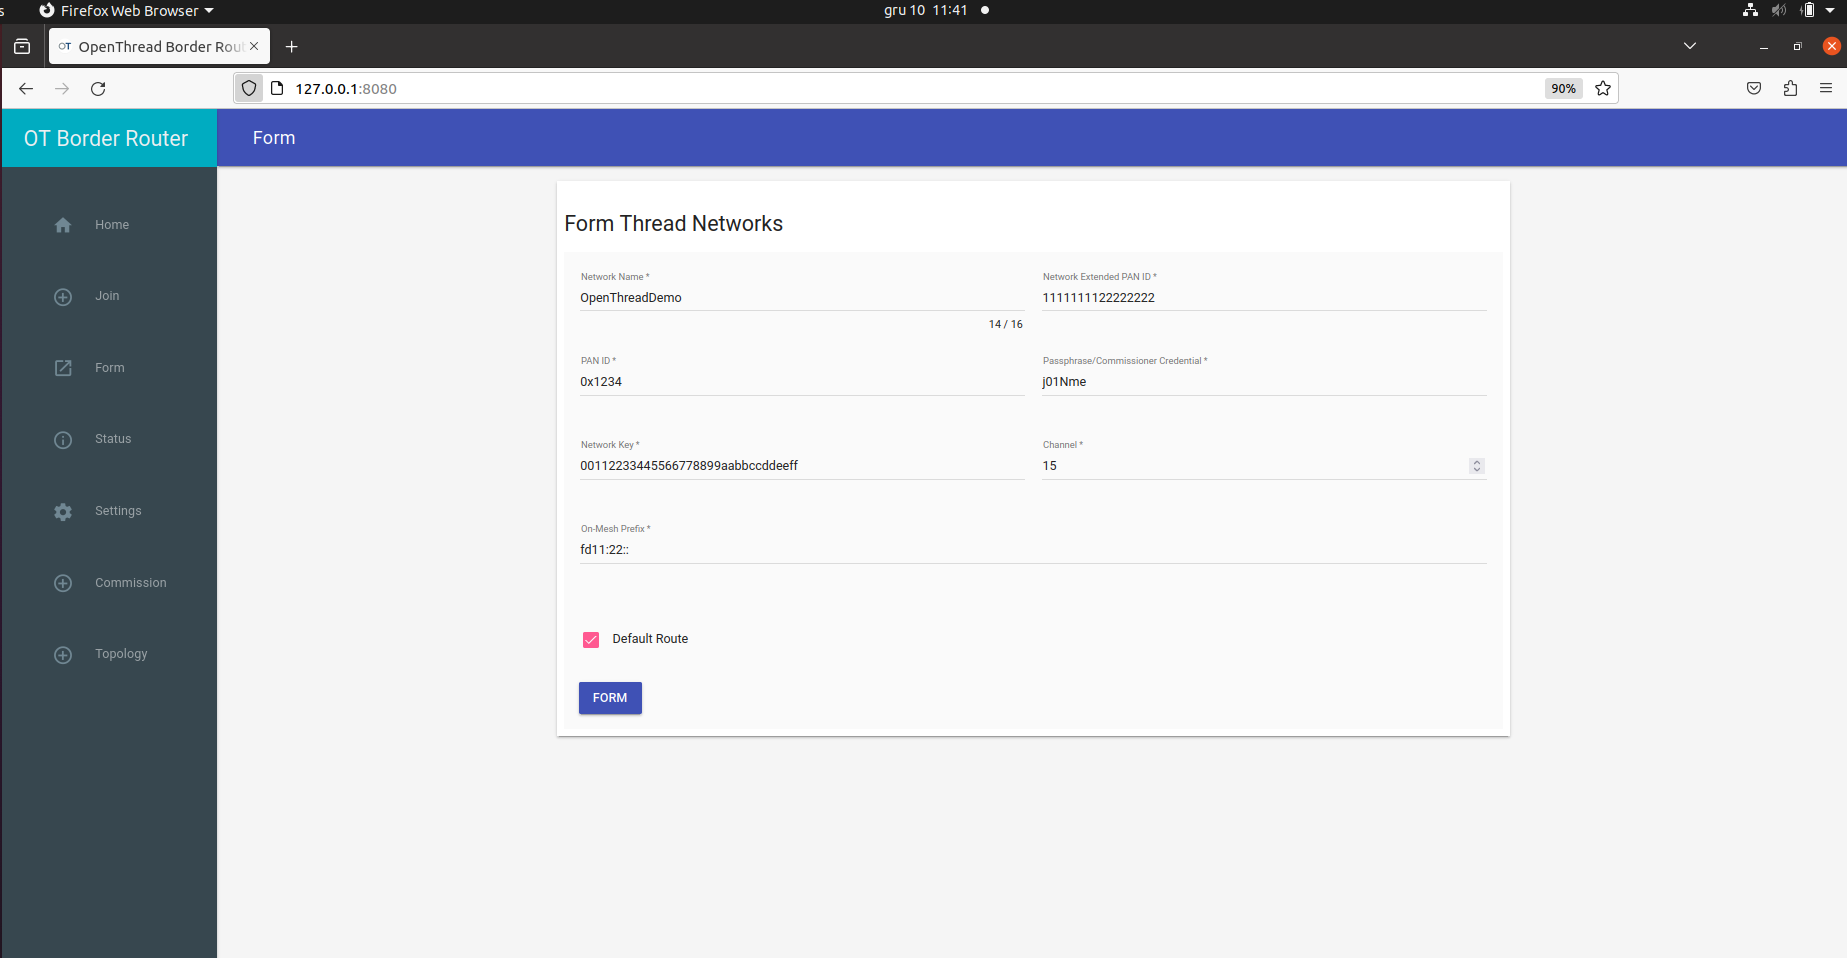
\includegraphics[width=0.8\linewidth]{graphics/screenshots/OTBR-web-gui.png}
    \caption{Zrzut ekranu interfejsu OTBR GUI z oknem do tworzenia sieci Thread.}
    \label{fig:otbr-web-gui}
\end{figure}

Wartości parametrów koniecznych do stworzenia sieci Thread, które opisano w Podsekcji \ref{subsec:network-forming}, przedstawiono w Tabeli \ref{tab:network-parameters}.

    \begin{table}[H]
    \centering
    \caption{Parametry sieci Thread.}
    \begin{tabular}{|l|l|}
        \hline
        \rowcolor{gray!20}
         \multicolumn{1}{|c|}{\textbf{Nazwa parametru}} & \multicolumn{1}{|c|}{\textbf{Wartość}}  \\
         \hline
         Network Name & pawel\_network \\
         \hline
         PAN ID & 0x0457 \\
         \hline
         Network Key & 00112233445566778899aabbccddeeff \\
         \hline
         Extended PAN ID & fb020000abcd0000 \\
         \hline
         Commissioning Credential & J01NME \\
         \hline
         Channel & 13 \\ 
         \hline
         Mesh-Local Prefix & fd11:22:: \\
         \hline
    \end{tabular}
    \label{tab:network-parameters}
\end{table}
    
Po zatwierdzeniu parametrów, a w konsekwencji utworzeniu sieci Thread, skonfigurowano Ruter brzegowy, aby pracował jako Commissioner w procesie przedstawionym w Podsekcji \ref{subsec:commissioning}. W tym celu wykorzystano OpenThread CLI \cite{otbr-cli}. Narzędzie to pozwala na konfigurację urządzeń sieci Thread, w których wdrożono OpenThread. Na Rysunku \ref{fig:ctl-commissioner} przedstawiono wprowadzone w konsolę OpenThread CLI komendy konfigurujące rolę Commissioner w Ruterze brzegowym oraz pozwalające na dołączenie do sieci wszystkim urządzeniom posiadającym Commissioning Credential o wartości \textit{J01NME}.
    
\begin{figure}[H]
    \centering
    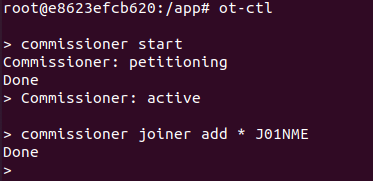
\includegraphics[width=0.8\linewidth]{graphics/screenshots/ot-ctl-commissioning.png}
    \caption{Zrzut ekranu konsoli OpenThread CLI, przedstawiający konfigurację roli Commissioner.}
    \label{fig:ctl-commissioner}
\end{figure}
    
Tak skonfigurowane urządzenie jest w pełni funkcjonalnym Ruterem brzegowym, pracującym w roli Commissioner.

W kolejnym kroku uruchomiono pozostałe platformy nRF52833 pracujące jak urządzenia FTD oraz HEATER i DIMMER. Po włączeniu urządzeń przystąpiono do konfiguracji roli Joiner każdego z węzłów.

Ukończywszy proces Commissioning, dokonano analizy powstałej topologi, dzięki której ustalono, że w sieci funkcjonują 2 węzły typu Dziecko, które pełnią role HEATER i  DIMMER, oraz 3 Rutery, z których jeden jest Liderem i Ruterem Brzegowym OTBR. Na potrzeby rozróżnienia 2 pozostałych Ruterów w dalszej części rozdziału, nadano im nazwę \textit{Router 1} oraz \textit{Router 2}. Następnie zweryfikowano połączenie między każdym węzłem sieci, rozsyłając pakiet ICMP (ang. \textit{Internet Control Message Protocol}) na adres multicast FF03::1, który jest subskrybowany przez każde urządzenie w danej sieci Thread. W Tabeli \ref{tab:mleid} zestawiono MLEID (ang. \textit{Mesh-Local Endpoint Identifiers}), czyli unikalne adresy IPv6 węzłów w utworzonej sieci Thread.

\begin{table}[H]
    \centering
    \caption{MLEID węzłów w sieci.}
    \begin{tabular}{|l|l|}
         \hline
         \rowcolor{gray!20}
         \multicolumn{1}{|c|}{Nazwa Węzła} & \multicolumn{1}{c|}{Adres IPv6} \\
         \hline
         OTBR & fd3f:cd2f:14fe:87f9:6b09:304e:878:6fb1 \\
         \hline
         HEATER & fd3f:cd2f:14fe:87f9:434d:bde5:7686:b429 \\
         \hline
         DIMMER & fd3f:cd2f:14fe:87f9:7998:c2a3:d56d:e3b0 \\
         \hline
         Router 1 & fd3f:cd2f:14fe:87f9:13a4:eced:d2c3:3922 \\
         \hline
         Router 2 & fd3f:cd2f:14fe:87f9:ce9e:4840:7dba:7356 \\
         \hline
    \end{tabular}
    \label{tab:mleid}
\end{table}


Upewniwszy się o poprawności funkcjonowania sieci, oraz że każde z urządzeń otrzymuje odpowiedź od pozostałych węzłów, uruchomiono aplikację System Controllera oraz Web GUI wykorzystując przygotowany wcześniej skrypt \textit{my-run-coap-server.sh} znajdujący się w repozytorium \cite{project-repo}. 

Topologię systemu po uruchomieniu wszystkich jego komponentów przedstawiono na Rysunku \ref{fig:system-topology}.

\begin{figure}[H]
    \centering
    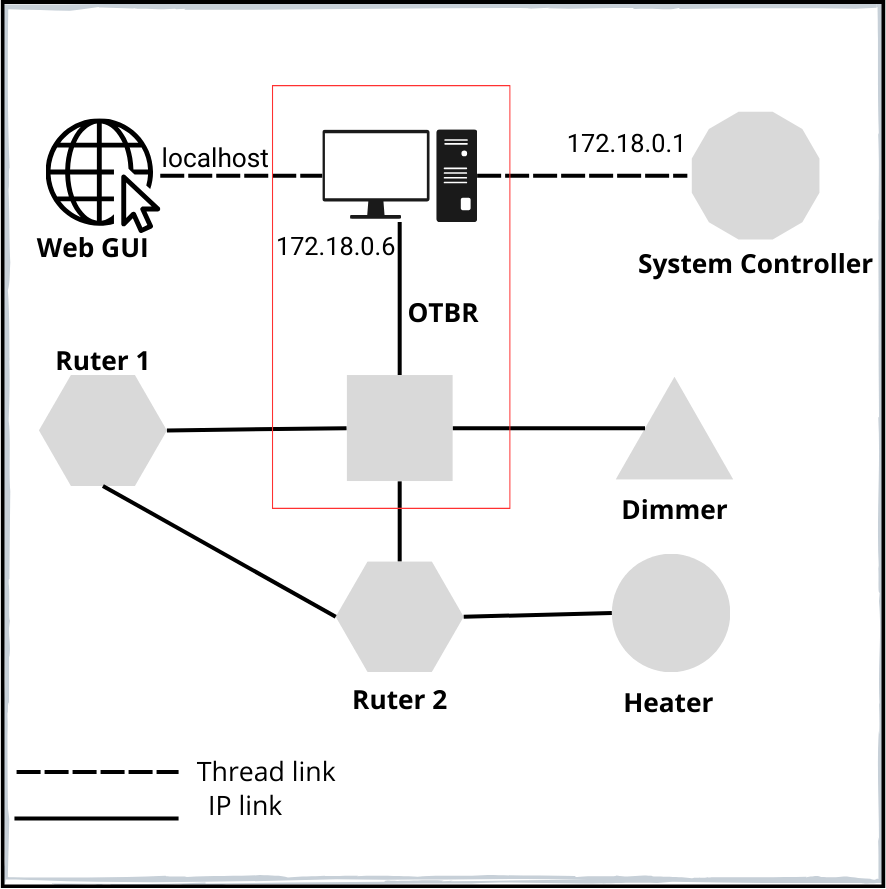
\includegraphics[width=0.8\linewidth]{graphics/system-topology.png}
    \caption{Topologia uruchomionego systemu.}
    \label{fig:system-topology}
\end{figure}

Ostatecznie włączono aplikację HEATER oraz DIMMER poprzez wciśnięcie przycisku Button 3 na obydwu urządzeniach. W efekcie zostało nawiązane połączenie klient-serwer między HEATER i DIMMER a System Controllerem.

Na Rysunku \ref{fig:serwer-app} zaprezentowano zrzut ekranu z konsoli, w której uruchomiono program System Controllera.

\begin{figure}[H]
    \centering
    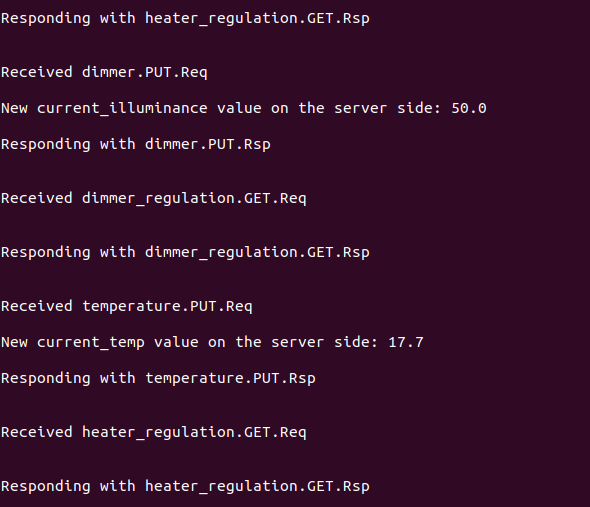
\includegraphics[width=0.8\linewidth]{graphics/screenshots/verification/system-controller-communication.png}
    \caption{Zrzut ekrany przedstawiający działanie System Controllera.}
    \label{fig:serwer-app}
\end{figure}

\section{Weryfikacja zasady działania systemu}

W celu weryfikacji poprawności zachowania stworzonego systemu wykorzystano narzędzie Grafana \cite{grafana}. Platforma Grafana pozwala na tworzenie interaktywnych paneli do monitorowania danych z wybranego przez użytkownika źródła, takiego jak baza danych. Aby zwizualizować dane pochodzące z logów systemowych, jako zasób wybrano zaimplementowaną Bazę Danych, której architektura przedstawiono na Rysunku \ref{fig:db-diagram}. Następnie z wykorzystaniem kwerend SQL utworzono panel Grafana zawierający 4 przebiegi czasowe, które przedstawiono na Rysunkach \ref{fig:graph-heater-temperature}, \ref{fig:graph-heater-regulation}, \ref{fig:graph-dimmer-illuminance},  \ref{fig:graph-dimmer-regulation}.
    
\begin{figure}[H]
    \centering
    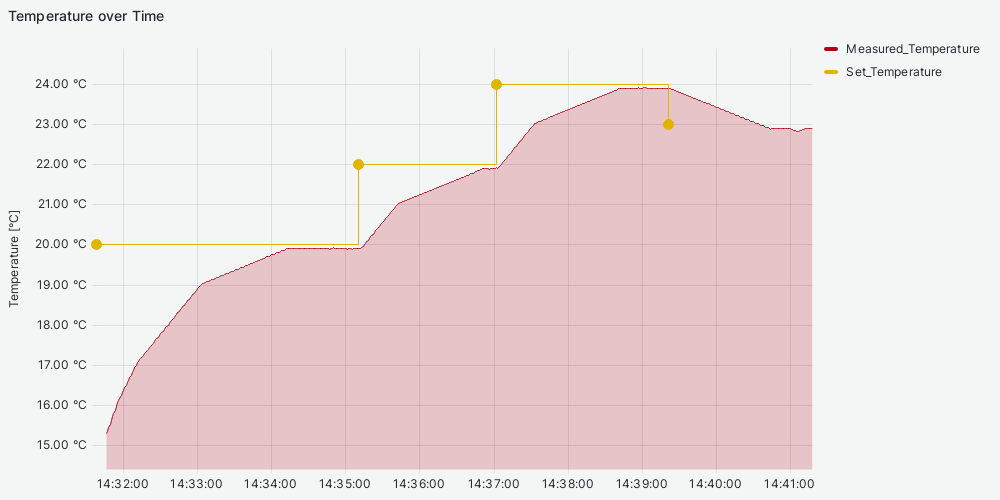
\includegraphics[width=0.8\linewidth]{graphics/grafana/temperature-lm.png}
    \caption{Przebiegi czasowe zmierzonej oraz ustalonej temperatury.}
    \label{fig:graph-heater-temperature}
\end{figure}

\begin{figure}[H]
    \centering
    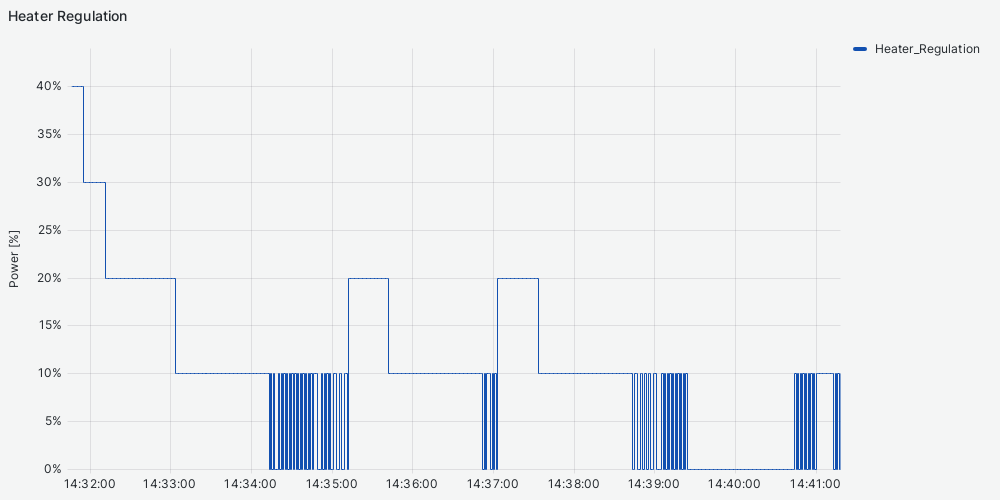
\includegraphics[width=0.8\linewidth]{graphics/grafana/heater-regulation-lm.png}
    \caption{Przebieg czasowy regulacji mocy układu HEATER.}
    \label{fig:graph-heater-regulation}
\end{figure}

\begin{figure}[H]
    \centering
    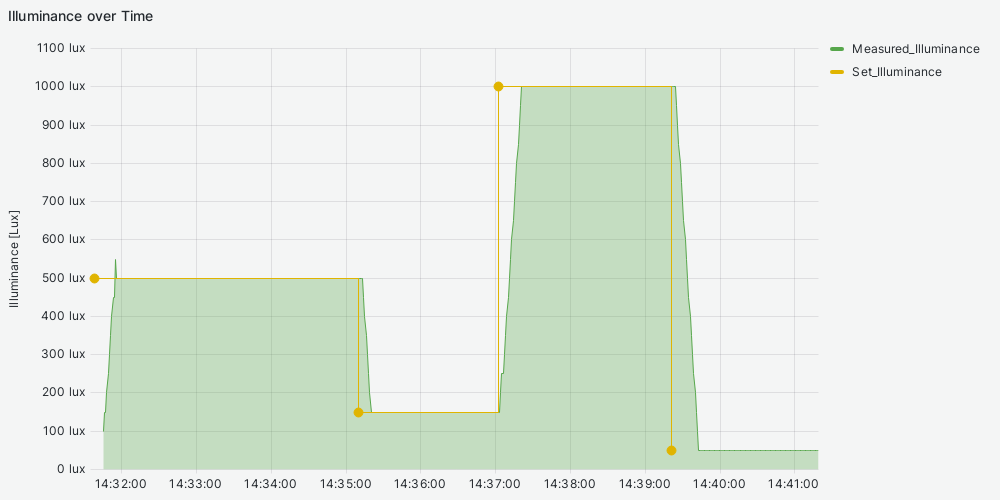
\includegraphics[width=0.8\linewidth]{graphics/grafana/illuminance-lm.png}
    \caption{Przebiegi czasowe zmierzonego oraz ustalonego natężenia oświetlenia.}
    \label{fig:graph-dimmer-illuminance}
\end{figure}

\begin{figure}[H]
    \centering
    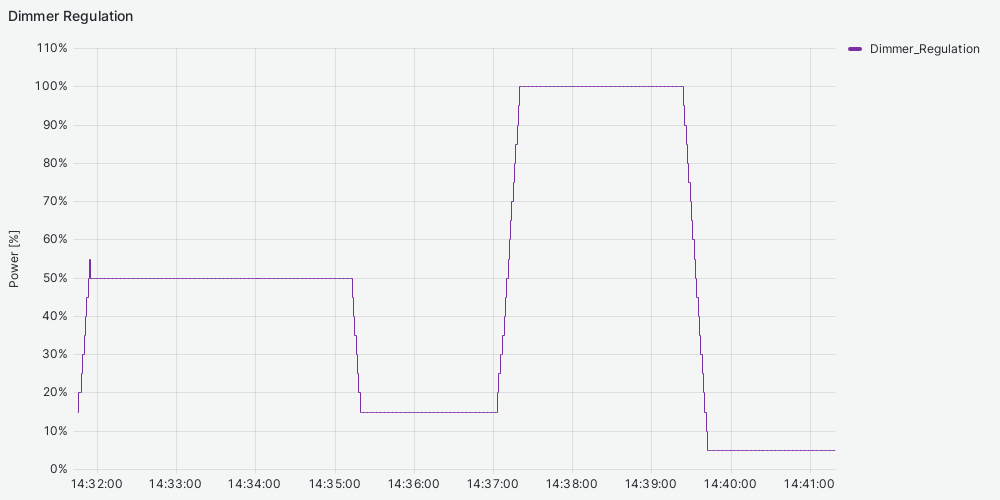
\includegraphics[width=0.8\linewidth]{graphics/grafana/dimmer_regulation-lm.png}
    \caption{Przebieg czasowy regulacji mocy układu DIMMER.}
    \label{fig:graph-dimmer-regulation}
\end{figure}
    
    Z przebiegów znajdujących się na Rysunku \ref{fig:graph-heater-temperature} oraz \ref{fig:graph-dimmer-illuminance} można zauważyć, że odpowiednio aktualna temperatura oraz natężenie oświetlenia zmierzają do ustalonej przez użytkownika wartości. Zobrazowane na Rysunkach \ref{fig:graph-heater-regulation} oraz \ref{fig:graph-dimmer-regulation} zmiany parametru regulacji pokrywają się ze zdefiniowanymi algorytmami w System Controllerze. Zatem, obserwując wszystkie 4 wymienione wykresy, można stwierdzić o poprawności działania systemu, względem poczynionych założeń. Na Rysunku \ref{fig:graph-heater-regulation} można zauważyć skokowe zmiany obliczanej wartości parametru regulacji, które są konsekwencją zauważonego w Sekcji \ref{subsec:system-behaviour} problemu, związanego z brakiem histerezy w zaimplementowanym algorytmie System Controllera.